\chapter{Mercoledì 13/05/2020}
Abbiamo introdotto la scorsa volta il gestore della concorrenza: abbiamo visto come in certi casi questo gestore neghi temporaneamente l'accesso al buffer a una transazione, precisamente quando non si hanno atteggiamenti seriali. Tutto ciò viene gestito attraverso operazioni di \emph{scheduling}: costruisco sequenze di operazioni R/W garantendo delle proprietà. Abbiamo, per esempio:
\[S1: r_1(x) r_2(z) w_1(x) w_2(z)\]
Dove le operazioni con $1$ sono eseguite dalla prima transazione e quelle con $2$ dalla seconda transazione. Il tutto è eseguito in \emph{interleaving}, cioè eseguiamo pezzi di transazione (nell'esempio le operazioni sono miste). Ribadiamo il ricorso ad algoritmi sofisticati!
\paragraph{Obiettivo} Evitare le anomalie
\paragraph{Soluzione} Scheduler. Come già detto consiste in un sistema che accetta o rifiuta, anche tramite riordino, le operazioni richieste dalle transazioni.
\paragraph{Schedule seriale} Uno schedule si dice seriale se per ogni transazione $t$, tutte le azioni di $t$ compaiono in sequenza, senza essere inframezzate da azioni di altre transazioni. Nel seguente schedule le transazioni vengono eseguite in sequenza
\[S2: r_0(x)r_0(y)w_0(x)r_1(y)r_1(x)w_1(y)r_2(x)r_2(y)r_2(z)w_2(z)\]
\paragraph{Schedule serializzabile} L'esecuzione di uno schedule $S_i$ è corretta quando produce lo stesso risultato di un qualunque schedule seriale $S_j$ definito dalle stesse transazioni di $S_i$.  Lo schedule $S_i$ è detto serializzabile.
\section{Nozioni di equivalenza}
\subsection{Relazione \emph{legge-da}}
Abbiamo le transazioni $i$ e $j$. Data un'operazione di lettura della prima $r_i(x)$ e un'operazione di scrittura della seconda  $w_j(x)$ presenti in uno schedule $S$ si dice che esiste una relazione (che noi chiameremo \emph{legge-da}) se:
\begin{itemize}
	\item l'operazione di scrittura $w_j(x)$ precede quella di lettura $r_i(x)$
	\item non si ha nessuna operazione di scrittura $w_k(x)$ tra di loro, con $k \neq j$.
\end{itemize}
Mi chiedo se l'operazione di lettura legge quanto ottenuto dall'operazione di scrittura o lo stato del database.
\paragraph{Scrittura finale} Definisco $w_i(x)$ in $S$ scrittura finale su $x$ se è l'ultima scrittura dell'oggetto $x$ nella schedule $S$.
\subsection{Schedule view-equivalenti} Due schemi sono \emph{view-equivalenti} se hanno:
\begin{itemize}
	\item le stesse relazioni \emph{legge-da} 
	\item le stesse scritture finali su ogni oggetto
\end{itemize}
\subsection{Schedule view-serializzabile} Uno schedule $S$ è detto \emph{view-serializzabile} se è \emph{view-equivalente} ad un qualche schedule seriale. L'insieme degli schedule view-serializzabili si indica con VSR. 

\subsection{Esempi}
\paragraph{Esempio con schedule view-serializzabili}
Consideriamo i seguenti schedule:
\begin{itemize}
	\item $S3:w_0(x)r_2(x)r_1(x)w_2(x)w_2(z)$
	\begin{itemize}
		\item Non seriale
		\item $r_2(x)$ e $r_1(x)$ leggono quanto scritto da $w_0(x)$. Dopo $w_2(x)$ non ho altre operazioni di lettura.
	\end{itemize}
	\item $S4:w_0(x)r_1(x)r_2(x)w_2(x)w_2(z)$
	\begin{itemize}
		\item Seriale
		\item Cambia l'ordine delle letture $r_1(x)$ e $r_2(x)$. Esse leggono quanto scritto da $w_0(x)$.
		\item Lo stato finale di $S3$ è lo stesso di $S4$. Le operazioni finali di scrittura sono le stesse
	\end{itemize}
	\item $S5:w_0(x)r_2(x)w_2(x)r_1(x)w_2(z)$
	\begin{itemize}
		\item Non seriale
		\item Le operazioni $r_1(x)$ e $r_2(x)$ non leggono più la stessa cosa: il primo legge quanto scritto da $w_0(x)$, il secondo quanto scritto da $w_2(x)$. Individuo che $S5$ non è sicuramente view-equivalente ad $S4$. Non stiamo dicendo che non è view-serializzabile.
	\end{itemize}
	\item $S6:w_0(x)r_2(x)w_2(x)w_2(z)r_1(x)$
	\begin{itemize}
		\item Seriale (non conta l'ordine delle transazioni ma se queste vengono interrotte da operazioni di altre transazioni per poi essere riprese)
		\item Confrontiamo con lo schedule precedente: le operazioni $r_2(x)$ e $r_1(x)$ leggono rispettivamente da $w_0(x)$ e $w_2(x)$ (come prima).
		\item Le operazioni di scrittura finale in $S5$ ed $S6$ sono le stesse: $w_2(x)$ e $w_2(z)$.
	\end{itemize}
\end{itemize}
Cosa possiamo dire?
\begin{itemize}
	\item La $S3$ è \emph{view-equivalente} allo schedule seriale $S4$ (quindi è view-serializzabile)
	\item $S5$ non è \emph{view-equivalente} allo schedule seriale $S4$, ma lo è rispetto allo schedule seriale $S6$ (quindi è view-serializzabile).
	\item Eseguo transazioni in modo diverso ma il risultato finale è lo stesso.
\end{itemize}
\paragraph{Esempi con schedule non view-serializzabili} 
\begin{itemize}
	\item \textbf{Perdita di aggiornamento}: $S3: r_1(x) r_2(x) w_1(x) w_2(x)$
	\begin{itemize}
		\item Sia $r_1(x)$ che $r_2(x)$ leggono lo stato del database
		\item Entrambe le transazioni leggono e scrivono lo stesso variabile.
		\item Qualunque ordine io faccia entrambe le transazioni leggono lo stesso valore di $x$: questa cosa in una situazione normale non è possibile. Per forza una delle due deve leggere il risultato dell'altra.
		\item Segue che questo schedule non è serializzabile.
	\end{itemize}
	\item \textbf{Letture inconsistenti}: $S4: r_1(x) r_2(x) w_2(x) r_1(x)$
	\begin{itemize}
		\item Ho una transazione che compie due operazioni di lettura: $r_1(x)$ due volte. L'altra transazione compie un'operazione di lettura $r_2(x)$ e una di scrittura $w_2(x)$
		\item L'unico ordinamento seriale con cui mi posso confrontare è quello in cui ottengo prima la transazione $1$ e poi la $2$. Quanto detto prima non può essere ricondotto a uno schedule seriale avente lo stesso risultato.
	\end{itemize}
	\item \textbf{Aggiornamento fantasma}: $S5: r_1(x) r_1(y) r_2(z) r_2(y) w_2(y) w_2(z) r_1(z)$
	\begin{itemize}
		\item La transazione $1$ legge $x$, legge $y$, legge $z$. La seconda transazione legge $z$, legge $y$, scrive $y$ e scrive $z$.
		\item Anche in questo caso non possiamo ricondurre lo schedule a un equivalente seriale con la stessa soluzione.
	\end{itemize}
\end{itemize}
Non sono \emph{view-serializzabili}, quindi non sono \emph{view-equivalenti} a nessun schedule seriale.
\subsection{Verifica della view-serializzabilità} Il gestore controlla se aggiungendo una certa operazione allo schedule si continua a rispettare i vincoli di ordinamento.
\begin{itemize}
	\item La complessità della verifica della view-equivalenza è polinomiale poichè devo scorrere tutto lo schedule. 
	\item Decidere la view-serializzabilità di uno schedule è un problema NP-Completo esponenziale! 
	\item Segue che l'algoritmo di verifica è troppo complicato.
\end{itemize}
Come risolviamo? Definiamo una condizione di equivalenza più ristretta, che non copra tutti i casi di equivalenza tra schedule coperti della view-equivalenza. Questa dovrà essere utilizzabile nella pratica, quindi avere una complessità inferiore.

\section{Conflitti tra operazioni}
Già con la view-equivalenza abbiamo visto un conflitto, precisamente tra una scrittura e una lettura successiva. Adesso vediamo anche altri tipi di conflitti tra due operazioni:
\begin{itemize}
	\item Una lettura seguita da una scrittura (conflitto \emph{read-write})
	\item Una scrittura seguita da una lettura (conflitto \emph{read-write})
	\item Una scrittura seguita da un'altra scrittura (conflitto \emph{write-write})
\end{itemize}
\paragraph{Definizione semplice di conflitto} Un'operazione $a_i$ è in conflitto con un'altra $a_j$ con $i\neq j$ se operano sullo stesso oggetto e almeno una di esse è una scrittura (nei casi precedenti c'è sempre un'operazione di scrittura). 
\paragraph{Conflict-equivalenza} Due schedule sono \emph{conflict-equivalenti} se
\begin{itemize}
	\item includono le stesse operazioni
	\item ogni coppia di operazioni in conflitto compaiono nello stesso ordine in entrambi gli schedule
\end{itemize}
\paragraph{Conflict-serializzabilità} Uno schedule è \emph{conflict-serializzabile} se è conflict-equivalente ad un qualche schedule seriale.
\paragraph{Confronto con la classe di schedule vista prima} Ricordiamo quanto detto prima parlando di \emph{verifica della view-serializzabilità}. Risulta dimostrabile che questa classe di schedule è strettamente contenuta nella classe degli schedule precedenti. Cosa significa tutto ciò?
\begin{itemize}
	\item Che ogni schedule conflict-serializzabile è anche view-serializzabile (CSR implica VSR)
	\item Che esistono schedule appartenenti a VSR che non appartengono a CSR.
\end{itemize}
\begin{center}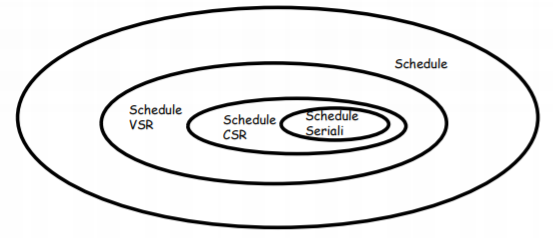
\includegraphics{images/159.PNG}\end{center}
\subsection{Verifica di conflict-serializzabilità} 
La verifica avviene attraverso il \emph{grafo dei conflitti}.
\begin{itemize}
	\item è orientato
	\item ogni nodo rappresenta una transazione
	\item un arco orientato va da $t_i$ a $t_j$ se c'è almeno un conflitto fra un'operazione $a_i$ e un'operazione $a_j$ tale che $a_i$ precede $a_j$.
\end{itemize}
\paragraph{Teorema} Uno schedule è in CSR se e solo se il grafico è aciclico!
\paragraph{Esempio di applicazione del teorema} Abbiamo la seguente schedule
\begin{center}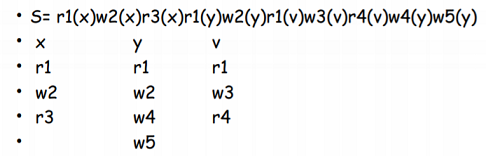
\includegraphics{images/160.PNG}\end{center}
Con le informazioni a disposizione disegno il seguente grafo
\begin{center}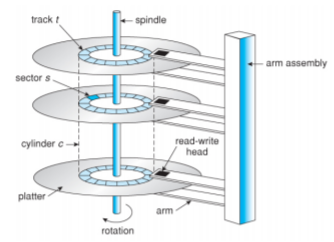
\includegraphics{images/161.PNG}\end{center}
\begin{itemize}
	\item Ho cinque transazioni, quindi disegno cinque nodi.
	\item Su ogni oggetto guardo l'ordine delle transazioni:
	\item in $x$:
	\begin{itemize}
		\item Ho $r1$ e $w2$, quindi conflitto che va dal nodo $1$ al nodo $2$. 
		\item Non ho conflitto tra nodo $1$ e nodo $3$ (due operazioni di lettura)
		\item Ho $w2$ ed $r3$, quindi conflitto che va dal nodo $2$ al nodo $3$
	\end{itemize}
	\item in $y$:
	\begin{itemize}
		\item Ho $r1$ e $w2$, conflitto già visto
		\item Ho $r1$ e $w4$, quindi conflitto da nodo $1$ a nodo $4$ 
		\item Ho $r1$ e $w5$, quindi conflitto da nodo $1$ a nodo $5$
		\item Ho $w2$ e $w4$, quindi conflitto da nodo $2$ a nodo $4$
		\item Ho $w2$ e $w5$, quindi conflitto da nodo $2$ a nodo $5$
		\item Ho $w4$ e $w5$, quindi conflitto da nodo $4$ a nodo $5$
	\end{itemize}
	\item in $v$:
	\begin{itemize}
		\item Ho $r1$ e $w3$, quindi conflitto da nodo $1$ a nodo $3$
		\item Ho $w3$ e $r4$, quindi conflitto da nodo $3$ a nodo $4$.
	\end{itemize}
\end{itemize}
Osservo che il grafo è aciclico. Segue che la schedule è conflict-serializzabile!
\paragraph{Esempio 2} Ulteriore esempio, preso dall'Atzeni, di conflict-equivalenza e di grafo dei conflitti
\begin{center}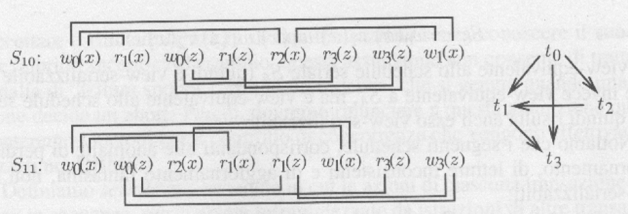
\includegraphics{images/228.PNG}\end{center}
\paragraph{Altri esempi} Vedere le diapositive della professoressa.
\paragraph{Succo del discorso} La conflict-serializzabilità è più rapidamente verificabile. Tuttavia necessità della costruzione, ogni volta, di un grafo dei conflitti (per ogni richiesta di scrittura). 
\subparagraph{Esempio di situazione problematica} Supponiamo di avere 100 transazioni al secondo, ciascuna accede a 10 pagine per la durata di 5 secondi. Ogni istante devo gestire grafi con 500 nodi tenendo traccia di oltre 5000 accessi delle 500 transazioni atttive. Il grafo si modifica dinamicamente tutte le volte e rende difficoltoso per lo scheduler prendere decisioni. Non è praticabile verificare l'aciclicità ad ogni richiesta di operazione.
\subparagraph{Cosa facciamo?} Ricerchiamo un nuovo metodo di accettazione delle richieste (scheduling) che mi garantisca a priori la conflict-serializzabilità (senza costruire un grafo tutte le volte).

\section{Lock, unlock e lock manager}
Alla base di questo nuovo metodo abbiamo il \emph{lock} e l'\emph{unlock}.
\begin{itemize}
	\item Ogni operazione di lettura è preceduta da \emph{lock} e seguita da \emph{unlock}.
	\item Ogni operazione di scrittura è preceduta da \emph{lock} e seguita da \emph{unlock}.
\end{itemize}
Il \emph{lock manager} è parte dello scheduler: accetta le richieste di lock e unlock. Applicare il \emph{lock} a una variabile significa renderla esclusivamente nostra, di una transazione in particolare. Dopo l'\emph{unlock} la variabile potrà essere utilizzata da altre transazioni.
\paragraph{Tipi di lock} Si distinguono due tipi di lock:
\begin{itemize}
	\item \textbf{lock condiviso}, per operazioni di lettura (r$\_$lock)
	\item \textbf{lock esclusivo}, per operazioni di scrittura (w$\_$lock)
\end{itemize}
Questi tipi di lock diversi, usati in momenti diversi sulla stessa risorsa, mi permettono di aumentare la concorrenza. Nel caso in cui una transazione prima legga e poi scriva un oggetto può:
\begin{itemize}
	\item richiedere subito un lock esclusivo, oppure
	\item chiedere prima un lock condiviso e poi uno esclusivo (\emph{lock upgrade})
\end{itemize}
\subsection{Comportamento dello scheduler}
Lo schedule agisce sfruttando la \emph{tavola dei conflitti}: conosce lo stato delle risorse e in base allo stesso decide se concedere o non concedere il \emph{lock} a una transazione.
\begin{itemize}
	\item se un lock viene concesso si dice che la risorsa è \emph{acquisita} dalla transazione
	\item nel momento dell'unlock la transazione \emph{rilascia} la risorsa.
\end{itemize}
\begin{center}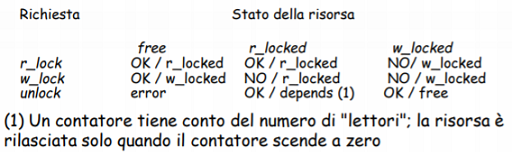
\includegraphics{images/162.PNG}\end{center}

\paragraph{Cosa succede se il lock viene negato?} La transazione viene messa da parte, in coda. Quando la risorsa è libera inizio a far scorrere la coda permettendo il lock!

\subsection{Ordine di lock e unlock} In questo momento stiamo garantendo solo la mutua esclusione sulla risorsa ma non la serializzabilità. Possiamo determinare l'ordine delle richieste di acquisizione e rilascio in modo da ottenere degli schedule CSR?
\paragraph{Locking a due fasi} Questo meccanismo mi permette di garantire la CSR a priori. La transazione, dopo aver rilasciato un lock, non può acquisirne altri finchè tutti quelli che ha acquisito non sono stati rilasciati! \textit{Accumulo, e poi rilascio senza acquisire altro}. 
\begin{center}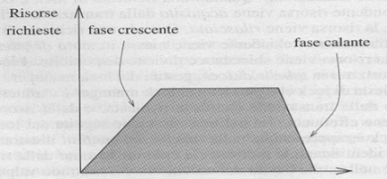
\includegraphics{images/165.PNG}\end{center}
Confrontiamo due schedule con le stesse operazioni: quello a destra non rispetta la 2PL, l'altro sì.
\begin{center}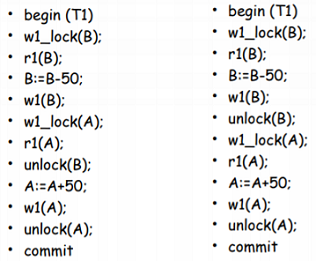
\includegraphics{images/164.PNG}\end{center}
Nell'esempio in 2PL inizio a fare unlock quando ho già fatto lock su tutti gli oggetti che mi servivano: prima di lavorare su B faccio unlock su A, poichè ho già finito con quell'oggetto. Lavoro su B e faccio unlock su B. Finchè non ho liberato B non potrò richiedere altri lock!
\paragraph{Upgrade e downgrade} L'upgrade può essere fatto solo nella fase di acquisizione, il downgrade nella fase di rilascio.
\paragraph{2PL e CSR} Esistono schedule in CSR, ma non in 2PL.
\begin{center}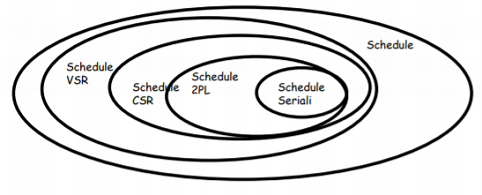
\includegraphics{images/166.PNG}\end{center}
\paragraph{Anomalie} Essendo in 2PL si risolvono anomalie di perdita di aggiornamento, di aggiornamento fantasma, e letture inconsistenti. Rimangono però delle anomalie, in particolare quella della \emph{lettura sporca}. Una transazione che a un certo punto fa abort va annullata: i valori intermedi potrebbero essere stati usati da altre transazioni. A questo punto dobbiamo dichiarare il fallimento di tutte le transazioni che hanno letto il valore scritto.
\begin{center}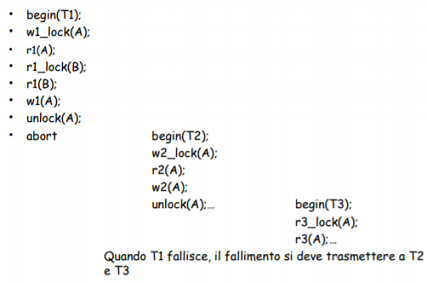
\includegraphics{images/167.PNG}\end{center}
Altro problema sono le attese incrociate (o \emph{deadlock}): due transazioni detengono ciascuna una risorsa e aspettano la risorsa detenuta dall'altra. In generale la probabilità di deadlock è bassa (inferiore a quella che si manifesti un conflitto) ma non nulla.
\begin{center}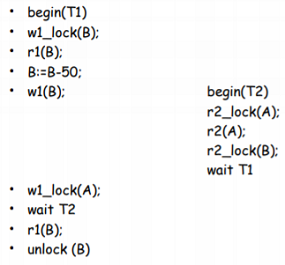
\includegraphics{images/168.PNG}\end{center}